\documentclass[tikz, margin=3mm]{standalone}
\usetikzlibrary{shadows}

\usepackage[T1]{fontenc}		% Selecao de codigos de fonte.
\usepackage[utf8]{inputenc}		% Codificacao do documento (conversão automática dos acentos)


\definecolor{silver}{HTML}{D6D6D6}
\usepackage{fontawesome}

\newcommand{\thehspace}{5.8cm}

\newcommand{\sethspace}[1]{
	\renewcommand*{\thehspace}{#1}
}

\newcommand{\disciplina}[6]{

    \noindent
    \begin{tabular}{l r}
        \multicolumn{2}{l}{\large\uppercase{\texttt{#1}} } \\ 
        \multicolumn{2}{p{\thehspace}}{\large\uppercase{\textbf{#2}}} \\ 
	\multicolumn{2}{l}{\large{\texttt{#3}}} \\
        \multicolumn{1}{p{\thehspace}}{\large\texttt{#4/#5}} & \large\texttt{(#6)} \\
    \end{tabular}
}


\begin{document}
    \begin{tikzpicture}[
every node/.style = {draw, fill=white, drop shadow, rounded corners},
every label/.append style = {
     label distance=1em,
     font=\scriptsize,
     every shadow/.style={opacity=0} % <- add this
  }
                        ]

\sethspace{6cm}

	\node [,]  (LOGICA) {\disciplina{TSII.101}{Lógica de \newline Programação}{\faUnlock}{40}{40}{4}};

	\node [, below of = LOGICA, node distance=3cm, ] (INGLES) {	\disciplina{TSII.102}{Produção de \newline Texto Técnico}{\faUnlock}{40}{---}{2}
};


\node[ below of = INGLES, node distance=3cm,] (SO)  {
	\disciplina{TSII.103}{Sistemas \newline Operacionais}{\faUnlock}{40}{40}{4}
};

\node[, below of = SO, node distance=3cm,  ] (WEBDESIGN)  {
	\disciplina{TSII.104}{Web Design}{\faUnlock}{40}{40}{4}
};


%jump
\node[, below of = WEBDESIGN, node distance=6cm, ] (EMPRESA)  {
	\disciplina{TSII.106}{Empreendedorismo}{\faUnlock}{30}{10}{2}
};


\node[, below of = EMPRESA, node distance=3cm,  ] (PROJ)  {
	\disciplina{TSII.107}{Projeto  Integrador I}{\faUnlock}{36}{04}{2}
};


\sethspace{6.5cm}

\node[, right of = INGLES, node distance=12cm, ] (BD)  {
	\disciplina{TSII.209}{Banco de Dados}{\faUnlock}{40}{40}{4}
};


\node[, below of = BD, node distance=3cm,  ] (REDES)  {
	\disciplina{TSII.105}{Redes de \newline Computadores}{\faUnlock}{40}{40}{4}
};


\node[, below of = REDES, node distance=3cm, ] (WEBI)  {
	\disciplina{TSII.211}{Desenvolvimento   WEB I}{\faLock~TSII.101, TSII.104}{40}{40}{4}
};


\node[, below of = WEBI, node distance=3cm,  ] (ES)  {
	\disciplina{TSII.210}{Engenharia de  \newline Software}{\faUnlock}{40}{40}{4}
};


%\node[, below of = WEBI, node distance=3cm,] (SERV)  {
%	\disciplina{TSII.212}{Servidores}{\faLock~TSII.105}{20}{20}{2}
%};

%\node[, right of = PROJ, node distance=12cm,   ] (PROJJ)  {
%	\disciplina{TSII.213}{Projeto    Integrador II}{\faLock~TSII.107}{36}{04}{2}
%};

%
%S3
\sethspace{6.8cm}

\node[, right of = LOGICA, node distance=25cm,] (POO)  {
	\disciplina{TSII.208}{Programação \newline Orientada a Objetos}{\faLock~TSII.101}{40}{40}{4}
};

\node[, below of = POO, node distance=6cm,] (SERV)  {
	\disciplina{TSII.212}{Servidores}{\faLock~TSII.105}{20}{20}{2}
};


\node[, below of  = SERV, node distance=6cm,] (APS)  {
	\disciplina{TSII.315}{Análise e Projeto  \newline de Sistemas}{\faLock~TSII.209, TSII.210}{20}{20}{2}

};

\node[, below of = APS, node distance=3cm,] (GESTAO)  {
	\disciplina{TSII.318}{Gestão de Projetos}{\faLock~TSII.106}{36}{04}{2}
};

\node[, below of = GESTAO, node distance=3cm ] (PROJJ)  {
	\disciplina{TSII.318}{Projeto Integrador II}{\faLock~TSII.213}{40}{72}{2}
	
};


%s04

\node[, right of = POO, node distance=12cm] (MOVEIS)  {
	\disciplina{TSII.314}{Programação para  \newline Dispositivos Móveis}{\faLock~TSII.208, TSII.209}{40}{80}{6}
};

\node[, below of = MOVEIS, node distance=6cm,] (SEG)  {
	\disciplina{TSII.212}{Seguran\c{c}a \newline de redes}{\faLock~TSII.105}{20}{20}{2}
};

\node[, below of = SEG, node distance=3cm,] (WEBII)  {
	\disciplina{TSII.316}{Desenvolvimento WEB II}{\faLock~TSII.208, TSII.209, TSII.211}{40}{40}{4}
};



\node[, below of = WEBII, node distance=9cm ] (PROJJJ)  {
	\disciplina{TSII.318}{Projeto Integrador III}{\faLock~TSII.213}{40}{72}{2}
	
};
%
%
%%% ligaduras
%
%
\draw[->, line width=0.05cm] (LOGICA) -- +(POO);
\draw[->, line width=0.05cm] (POO) -- +(MOVEIS);
\draw[->, line width=0.08cm,  dashed ] (LOGICA) to[out=355, in=174]  (WEBI);
\draw[->, line width=0.05cm] (BD) - |(MOVEIS);
\draw[->, line width=0.08cm,  loosely dashdotted] (BD) to[out=5,in=185]   (APS);
\draw[->, line width=0.08cm, loosely dashdotted] (APS) to[out=355,in=186]  (WEBII);
\draw[->, line width=0.05cm] (WEBDESIGN) -- +(WEBI);
\draw[->, line width=0.05cm] (WEBI) -- +(WEBII);
\draw[->, line width=0.05cm, ] (ES) -- +(APS);
\draw[->, line width=0.05cm] (REDES) -- +(SERV);
\draw[->, line width=0.05cm] (SERV) -- +(SEG);
%\draw[->, line width=0.05cm] (SERV) to[out=240, in=60] (WEBII);
\draw[->, line width=0.08cm, dashed] (POO) to[out=355, in=174]  (WEBII);
\draw[->, line width=0.05cm] (EMPRESA) -- +(GESTAO);
\draw[->, line width=0.05cm] (PROJ) -- +(PROJJ);
\draw[->, line width=0.05cm] (PROJJ) -- +(PROJJJ);


% LABELS


\node[above of = LOGICA, node distance = 3cm,   text width=7.4cm, fill=black] { 

\begin{tabular}{l}

	\\
		\textcolor{white}{\Large\bfseries  ~~PRIMEIRO SEMESTRE }\\
	\textcolor{white}{\LARGE\bfseries ~\quad\quad }\\
	\end{tabular}

};

\node[above of = BD, node distance = 6cm,   text width=8.1cm, fill=black] { 

\begin{tabular}{l}

	\\
		\textcolor{white}{\Large\bfseries~\quad\,SEGUNDO SEMESTRE }\\
	\textcolor{white}{\LARGE\bfseries ~\quad\quad }\\
	\end{tabular}

};


\node[above of = POO, node distance = 3cm,   text width=8.4cm, fill=black] { 
	\begin{tabular}{l}

	\\
		\textcolor{white}{\Large\bfseries  ~\quad\,TERCEIRO SEMESTRE }\\
	\textcolor{white}{\LARGE\bfseries ~\quad\quad }\\
	\end{tabular}
};


\node[above of = MOVEIS, node distance = 3cm,   text width=8.4cm, fill=black] { 
	\begin{tabular}{l}

	\\
		\textcolor{white}{\Large\bfseries  ~\quad\,QUARTO SEMESTRE }\\
	\textcolor{white}{\LARGE\bfseries ~\quad\quad }\\
	\end{tabular}
};



\node[gray,  text width=2.5\textwidth, text height=0.4cm, fill=silver] (OPT)  at (11.3, -21) { 
\centering 
\\
\textcolor{black}{\LARGE\bfseries\,OPTATIVAS }
\\	\,
\,
};



\node[black, text width=3.8\textwidth, text height=0.4cm,  fill=black] (M) at (18.75, 6) { 
\centering 
\\
\textcolor{white}{\LARGE\bfseries\,OBRIGAT\'ORIAS }
\\	\,
\,
};


%% Optativas
%
\sethspace{5.8cm}




\node[rounded corners, below of = OPT, node distance=3cm, ] (ARTES)  {
	\disciplina{TSII.402}{Educação Física}{\faUnlock}{15}{25}{2}

};


\node[rounded corners, left of = ARTES, node distance=11.5cm, ] (EDF)  {
	\disciplina{TSII.401}{Artes}{\faUnlock}{20}{20}{2}

};

\node[rounded corners, right of = ARTES, node distance=11.5cm, ] (LIBRAS)  {
	\disciplina{TSII.403}{Libras}{\faUnlock}{20}{20}{2}

};



\node[label={\huge\textbf{LEGENDA}},  below of= PROJJJ , xshift=-4em , node distance=5.6cm, text width=11.4cm] (kkkk)  {
	
    \noindent
    \fontsize{12pt}{10pt} 
    \renewcommand{\arraystretch}{1.5}
    \begin{tabular}{l r}
	\multicolumn{2}{l}{\large\texttt{Código da disciplina}}  \\ 
        \multicolumn{2}{l}{\large\textbf{NOME DA DISCIPLINA}} \\ 
        \multicolumn{2}{l}{\large\faLock~\texttt{Código dos pré-requisitos ou \faUnlock~sem pré-requisitos} }  \\
        \large\texttt{CH teórica/prática}  & \large\texttt{(Número de créditos)} \\
        
    \end{tabular}
};


    \end{tikzpicture}
\end{document}